\chapter{History of Equity Markets}

\section{Introduction}
This chapter explores the relationships between risk and return.\\

The fundamental concept is simple: as investors take on more risk, they expect a higher return. This is the risk-return trade-off.\\


\section{Math for Returns}

\begin{definitionbox}{Purchase of a Share}
    At the end of a period of owning a share, the return consists of two components: the dividend paid out during the period and the value of the share at the end.
    
    The final share price of a stock is the sum of the dividend paid at time $t+1$ and the price of the stock at time $t+1$.
    \begin{equation}
        \text{Share Price} = Div_{t+1} + P_{t+1}
    \end{equation}

    The percentage return can be calculated using the formula:
    \begin{equation}
        R_{t+1} = \frac{Div_{t+1} + P_{t+1} - P_t}{P_t}
    \end{equation}
\end{definitionbox}

\begin{definitionbox}{Dividend Yield and Capital Gain}
    Rearranging the percentage return formula, we can express the return as the sum of the dividend yield and the capital gain:
    \begin{equation}
        R_{t+1} = \frac{Div_{t+1} + P_{t+1} - P_t}{P_t}  = \frac{\overbrace{Div_{t+1}}^{\text{Dividend Yield}}}{P_t} + \frac{\overbrace{P_{t+1} - P_t}^{\text{Capital Gain}}}{P_t}
    \end{equation}

    The dividend yield is the income earned per dollar invested, and the capital gains is the percentage change in the price of the security over the given period, accounting for the growth of the investment's value.
\end{definitionbox}

\begin{definitionbox}{Nominal and real return}
    Used to measure investment performance. The nominal return is the percentage change in the value of an investment over a given period expressed in nominal terms, the currency of the investment.\\
    
    Real return is the nominal return adjusted for inflation. It considers the purchasing power of the investment, accounting for the change in the price level of goods and services.\\

    Inflation can represented with a price index, called the CPI, or consumer price index. It reflects the average price of a basket of goods bought in the economy over a year. Another index, the retail price index (RPI) can be used, which reflects the average price of a typical basket of goods purchased by an average household.\\

    The real return can be calculated using the formula, where $I_t$ is the price index at time $t$:
    \begin{equation}
        R^R_{t+1} = \frac{\frac{Div_{t+1} + P_{t+1}}{I_{t+1}}}{P_t / I_t} - 1
    \end{equation}

    We can rewrite as such, where $h_{t+1}$ is the inflation rate at time $t+1$:
    \begin{equation}
        R^R_{t+1} = (R_{t+1} + 1)(1-h_{t+1}) - 1
    \end{equation}

    We can ignore second order terms, and approximate the real return as:
    \begin{equation}
        R^R_{t+1} \approx R_{t+1} - h_{t+1}
    \end{equation}

\end{definitionbox}


\begin{definitionbox}{The Arithmetic and Geometric Mean}
    The arithmetic mean is the return earned in an average period over the entire investment duration, defined by:

    \begin{equation}
        \bar{R} = \frac{1}{N} \sum_{t=1}^{N} R_t
    \end{equation}



    The geometric mean takes into account the compounding effect, which is more apparent over longer time periods. So it calculates the average compound return per period over the investment duration of $N$ periods, defined by:

    \begin{equation}
        \bar{R}^G = \left( \prod_{t=1}^{N} (1 + R_t) \right)^{\frac{1}{N}} - 1
    \end{equation}


\end{definitionbox}



\begin{examplebox}{Averages Example}
    Consider the following data:
    \begin{itemize}
        \item Year 1: 5\%
        \item Year 2: -3\%
        \item Year 3: 12\%
    \end{itemize}

    The arithmetic average is:
    \begin{equation}
        \bar{R} = \frac{1}{3} (5 - 3 + 12) = 4.67\%
    \end{equation}

    The geometric average is:
    \begin{equation}
        \bar{R}^G = \left( (1 + 0.05)(1 - 0.03)(1 + 0.12) \right)^{\frac{1}{3}} - 1 = 4.67\%
    \end{equation}
\end{examplebox}



\section{Indices and Correlations}

This section gives an exercise to calculate the monthly returns and volatility of three return series, the FTSE 100, the S\&P 500, and the US-10 year bond, followed by calculating correlations.

\begin{sidenotebox}{Volatility}
    The volatility of a return series is a measure of the dispersion of the returns around the mean. It is calculated as the standard deviation of the returns.\\

    The standard deviation is calculated as:
    \begin{equation}
        \sigma = \sqrt{\frac{1}{N} \sum_{t=1}^{N} (R_t - \bar{R})^2}
    \end{equation}
\end{sidenotebox}

\begin{sidenotebox}{Correlation}
    The correlation coefficient measures the strength and direction of a linear relationship between two variables. It ranges from -1 to 1.\\

    A correlation of 1 indicates a perfect positive linear relationship, -1 indicates a perfect negative linear relationship, and 0 indicates no linear relationship.\\

    The correlation coefficient $\rho_{X,Y}$ which represents the correlation between variables $X$ and $Y$, calculated as:
    \begin{equation}
        \rho_{X,Y} = \frac{\cov(X,Y)}{\sigma_X \sigma_Y}
    \end{equation}

    Where $\cov(X,Y)$ is the covariance of $X$ and $Y$, and $\sigma_X$ and $\sigma_Y$ are the standard deviations of $X$ and $Y$ respectively.\\

    The covariance is calculated as:
    \begin{equation}
        \cov(X,Y) = \E[(X - \E[X])(Y - \E[Y])]
    \end{equation}
    This would be calculated as the following summation:
    \begin{equation}
        \cov(X,Y) = \frac{1}{N} \sum_{t=1}^{N} (X_t - \bar{X})(Y_t - \bar{Y})
    \end{equation}

    

    It is quite common to denote correlations between securities using a correlation matrix, where the diagonal elements are 1, and the off-diagonal elements are the correlation coefficients.\\

    Note that $\rho_{X,Y} \equiv \rho_{Y,X}$, so this matrix is symmetric.\\
    
    The correlation matrix is calculated as:
    \begin{equation}
        \mb{C} = \left( \begin{array}{c|ccc}
        & \text{Security 1} & \text{Security 2} & \text{Security 3} \\ \hline
        \text{Security 1} & 1 & \rho_{1,2} & \rho_{1,3} \\
        \text{Security 2} & \rho_{2,1} & 1 & \rho_{2,3} \\
        \text{Security 3} & \rho_{3,1} & \rho_{3,2} & 1 
        \end{array} \right)
    \end{equation}

    An example of what a correlation matrix might look like is:
    \begin{equation}
        \mb{C} = \begin{bmatrix}
            1 & 0.8 & 0.3 \\
            0.8 & 1 & 0.5 \\
            0.3 & 0.5 & 1
        \end{bmatrix}
    \end{equation}

\end{sidenotebox}

\section{Risk and Return}
\begin{itemize}
    \item Generally, higher risk is associated with potential for higher returns, as seen in equities, whereas lower risk investments like bonds offer more modest returns with less volatility.
    \item Historical data highlights that equities typically provide higher average returns but also greater volatility, exposing investors to potential significant losses.
    \item Conversely, less risky assets like government bonds or money market funds yield lower returns but ensure greater stability and are preferred for income preservation.
    \item Analyzing capital market returns shows that stocks exhibit the highest average returns and volatility, while treasuries yield the lowest, reinforcing the positive correlation between risk and return.
\end{itemize}

In Table \ref{tab:risk_return_tradeoff}, we see the risk-return tradeoff for various investments. Note that for the U.S. Treasury Bills, the average return and standard deviation values (bolded) are very low compared to other returns and standard deviations. 
\begin{table}[ht]
    \centering
    \caption{Risk-Return Tradeoff: Geometric Average Returns (1926-2020)}
    \label{tab:risk_return_tradeoff}
    \begin{tabular}{@{}lcc@{}}
    \toprule
    \textbf{Investment} & \textbf{Average Return/Mean Return} & \textbf{Standard Deviation} \\ \midrule
    Small stocks        & 12.52\%                 & 33.16\%                    \\
    S\&P 500            & 10.52\%                 & 19.81\%                    \\
    Corporate bonds     & 7.02\%                  & 8.15\%                     \\
    U.S. Treasury bonds & 5.39\%                  & 8.38\%                     \\
    U.S. Treasury bills & \textbf{3.61\% }        &\textbf{ 3.16\% }           \\
    CPI                 & 3.03\%                  & 1.76\%                     \\ \bottomrule
    \end{tabular}
\end{table}

The relations are better illustrated in a risk-return tradeoff graph, as seen in Figure \ref{fig:risk_return}.

\begin{figure}[H]
    \centering
    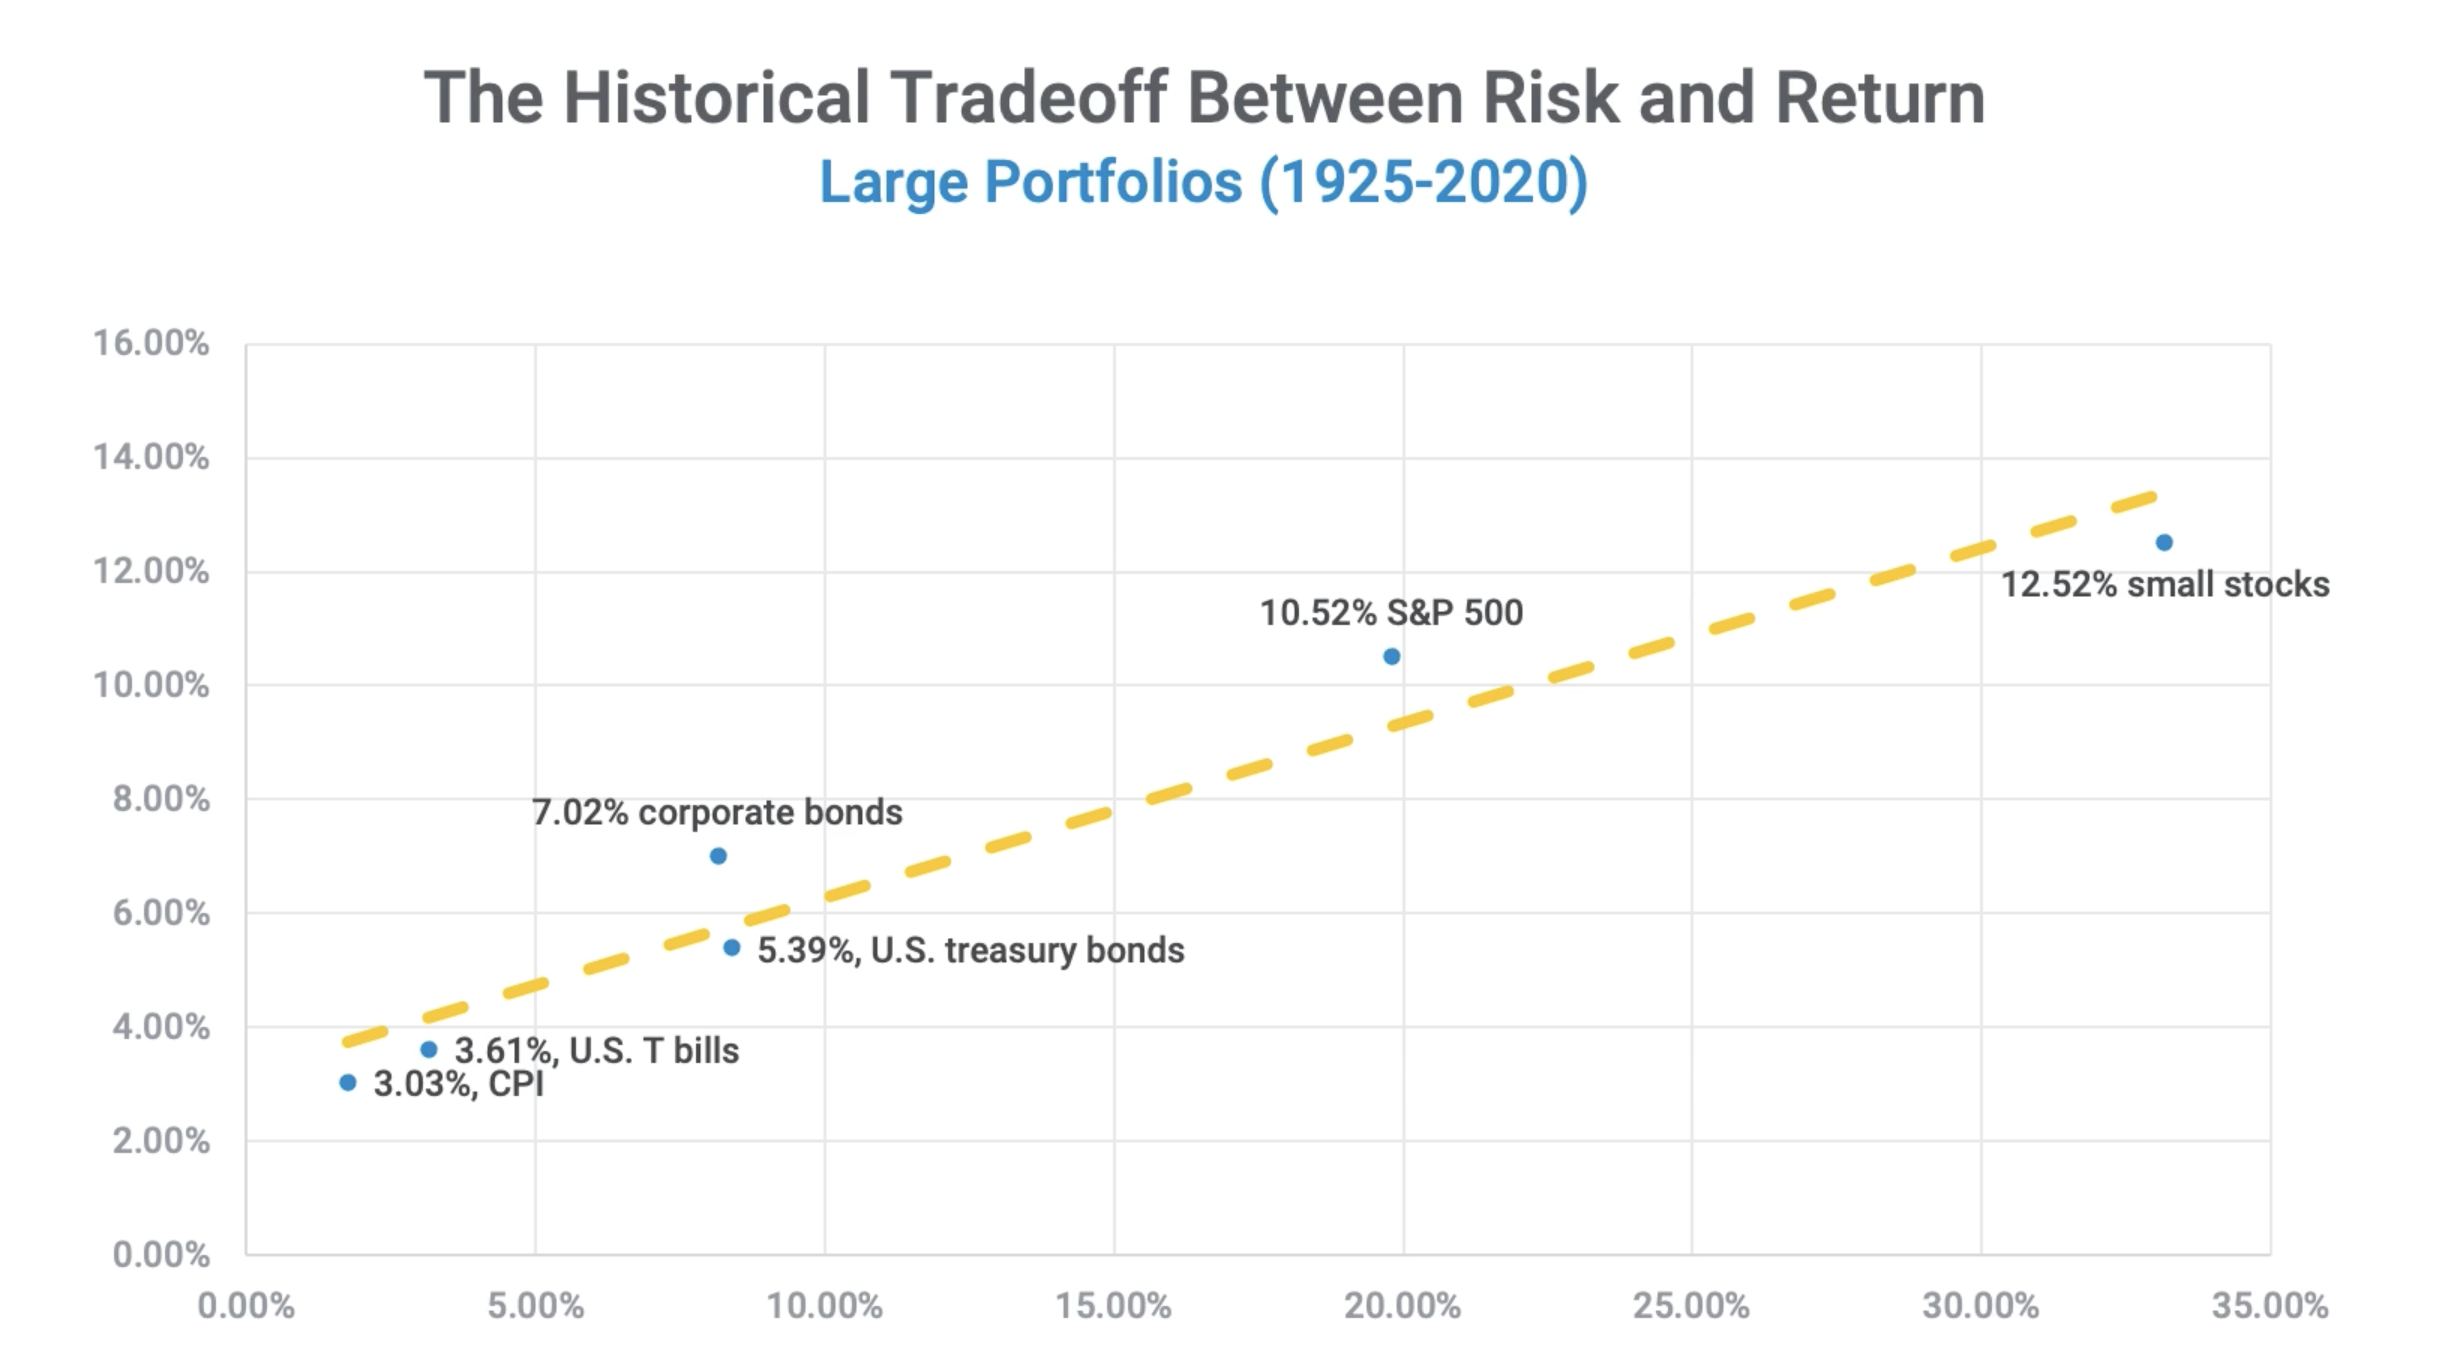
\includegraphics[width=0.8\textwidth]{img/5.4.png}
    \caption{Historical Tradeoff between Risk and Return}
    \label{fig:risk_return}
\end{figure}

\section{Live Tutorial}


\begin{table}[]
    \centering
    \small
    \caption{Summary of Financial Data of a Fictional Company (numbers in '000s)}
    \label{tab:fin_data_live}
    \begin{tabular}{@{}lllllll@{}}
    \toprule
    \textbf{Year (FY end in December)} & \textbf{2023A} & \textbf{2024P} & \textbf{2025P} & \textbf{2026P} & \textbf{2027P} & \textbf{2028P} \\ \midrule
    Revenue Growth Rate                  &           & 15.00\%     & 10.00\%   & 8.00\%        & 6.00\%    & 5.00\%      \\\midrule
    Revenues in \$m                    & 190,000.0      & 218,500.0      & 240,350.0      & 259,578.0      & 275,152.7      & 288,910.3      \\
    EBIT (Operating) margin              & 42.11\%   & 42.50\%     & 42.50\%   & 42.50\%       & 43.50\%   & 42.50\%     \\
    EBIT (Operating income)            & 80,000.0       & 92,862.5       & 102,148.8      & 110,320.7      & 116,939.9      & 122,786.9      \\
    Effective Tax Rate                   & 16.50\%   & 16.50\%     & 16.50\%   & 16.50\%       & 16.50\%   & 16.50\%     \\\midrule
    EBIT(1-t)                            & 66,800.0  & 77,540.2    & 85,294.2  & 92,117.7      & 97,644.8  & 102,527.0   \\
    - Capex                              & -24,000.0 & -27,600.0   & -30,360.0 & -32,788.8     & -34,756.1 & -36,493.9   \\
    + Depreciation                       & 14,000.0  & 16,100.0    & 17,710.0  & 19,126.8      & 20,274.4  & 21,288.1    \\
    \textbf{- Change in NWC*}            &           & -3,675.0    & -2,817.5  & -2,479.4      & -2,008.3  & -1,774.0    \\\midrule[2pt]
    FCFF                                 &           & 62,365.2    & 69,826.7  & 75,976.3      & 81,154.8  & 85,547.2    \\
    - FCFF for 01/2024                   &           & -5,197.1    &           &               &           &             \\
    FCFF excluding 01/2024               &           & 57,168.1    & 69,826.7  & 75,976.3      & 81,154.8  & 85,547.2    \\\midrule[2pt]
    \textbf{Cost of capital (WACC) **}              &           & 10.92\%     & 10.92\%   & 10.92\%       & 10.92\%   & 10.92\%     \\\midrule[2pt]
    Number of years from 'NOW'           &           & 0.92        & 1.92      & 2.92          & 3.92      & 4.92        \\
    Cumulated discount factor            &           & 0.91        & 0.82      & 0.74          & 0.67      & 0.60        \\
    PV(FCFF)                             &           & 51,989.0    & 57,251.6  & 56,163.4      & 54,087.5  & 51,404.1    \\ \midrule
    Terminal Value (TV)                  &           &             &           &               &           & 1,518,507.1 \\
    PV (TV)                              &           & 912,448.5   &           &               &           &             \\
    Enterprise Value = Sum of PV         &           & 1,183,344.1 &           & 77\% TV as EV &           &             \\
    - Net Debt                           &           & -50,000.0   &           &               &           &             \\
    Value of Equity                      &           & 1,133,344.1 &           &               &           &             \\
    Number of Shares in millions         &           & 7,500.0     &           &               &           &             \\
    Implied Share Price                  &           & \textbf{151.11  }    &           &               &           &             \\
    Current Share Price as of 12/02/2024 &           & 200         &           &               &           &             \\
    Overrvalued by                       &           & \textbf{32.35\% }    &           &               &           &             \\ \bottomrule
    \end{tabular}
    \end{table}



    \begin{table}[ht]
        \centering
        \caption{Summary of Changes in Net Working Capital* (numbers in '000s)}
        \label{tab:nwc_summary}
        \begin{tabular}{@{}lrrrrrr@{}}
        \toprule
        \textbf{Description} & \textbf{2023A} & \textbf{2024P} & \textbf{2025P} & \textbf{2026P} & \textbf{2027P} & \textbf{2028P} \\
        \midrule
        A/R               & 40,000.0 &       &       &       &       &       \\
        Inventory         & 3,500.0  &       &       &       &       &       \\
        A/P               & -19,000.0&       &       &       &       &       \\
        \midrule
        NWC               & 24,500.0 & 28,175.0 & 30,992.5 & 33,471.9 & 35,480.2 & 37,254.2 \\
        $\Delta$ in NWC   & 3,675.0  & 2,817.5 & 2,479.4 & 2,008.3  & 1,774.0  &       \\
        \bottomrule
        \end{tabular}
    \end{table}

\begin{table}[ht]
    \centering
    \caption{WACC ** (numbers in '000s)}
    \label{tab:wacc}
    \begin{tabular}{@{}lc@{}}
    \toprule
    \textbf{Metric}                     & \textbf{Value}    \\
    \midrule
    Cost of Debt                        & 5.00\%            \\
    Effective Tax Rate                  & 16.50\%           \\
    Total Debt                          & \$55,000.00       \\
    Cash \& Short-term Inv.             & \$5,000.00        \\
    Net Debt                            & \$50,000.00       \\
    After Tax Cost of Debt              & 4.18\%            \\
    Risk Free Rate                      & 4.00\%            \\
    Beta                                & 1.02              \\
    Market Risk Premium                 & 7.00\%            \\
    Cost of Equity                      & 11.14\%           \\
    MV of Equity on 12/02/2024          & \$1,500,000.00    \\
    D/V                                 & 3.2\%             \\
    E/V                                 & 96.8\%            \\
    WACC                                & 10.92\%           \\
    \bottomrule
    \end{tabular}
\end{table}

\begin{itemize}
    \item Whole point of the DCF: determine if the company is undervalued or overvalued. We only intend to buy underpriced stocks.
    \begin{itemize}
        \item Some questions to ask:
        \item How is it doing in comparison to competitors?
        \item Cross-selling opportunities? A cross-selling opportunity is when a company sells a different product or service to an existing customer.
        \item Any planned mergers or acquisitions?
    \end{itemize}
    \item Start with the income statement.
    \item Then make assumptions on:
    \item \textbf{Revenue Growth: } (Table \ref{tab:fin_data_live})
        \begin{itemize}
            \item There was double-digit growth forecasted from 2023-2025, but it cannot be sustained forever. DCF cannot forecast an infinite number of cash flows forever. So let 2028 be the terminal year, and it will cap at a 5\% growth rate.
            \item This capped growth rate usually has an upper limit equal to the GDP growth rate of the company's country. This could differ if the company is a multinational one.
        \end{itemize}
    \item \textbf{Operating Margins: } (Table \ref{tab:fin_data_live})
        \begin{itemize}
            \item After determining the revenue growth assumptions, next estimate the \textbf{operating margins}.
            \item  There are different margins, such as the profit margin, EBIT, etc.
            \item Currently for 2023 it is \textbf{42.11\%}. Assume it has no plans for expansion, so the margin will remain constant.
            \item Let's also assume this fictional is a service company, so it also does not have much room for improvement in margins.
            \item When determining this, it is important to look into the company's expansion strategy.
        \end{itemize}
    \item \textbf{EBIT or Operating Income: } (Table \ref{tab:fin_data_live})
    \begin{itemize}
        \item Assume tax rate remains constant at 16.5\%. Using the marginal or statutory tax rates (values which are provided by tax authorities) are generally higher, so companies are highly incentivised to not pay them and can avoid paying all of the taxes, by using strategies like tax havens, depreciation of assets as a non-cash expense, tax credits, deducting interest expenses from debt financing (companies are not taxed on debt).
        \item We've assumed it to remain constant at 16.5\%. 
        \item Also, when decided tax rates, do not account for outliers (spikes) as they are likely one-time events.
        \item \textbf{EBIT(1-t)} is also known as NOPAT, net operating profit after tax.  
    \end{itemize}
    \item \textbf{Other Assumptions: } (Table \ref{tab:fin_data_live})    
    \begin{itemize}
            \item Assume \textbf{CAPEX} grows with revenue (likely if the company is at maximum capacity, and likes to expand). However, if you're aware a company is cost-cutting, then CAPEX can decrease.
            \item \textbf{Depreciation} is also assumed to increase with revenue (because there is more investment in assets like machinery, buildings, etc.)
            \item $CAPEX - Depreciation = Net \ Investment$ and this value always must be positive.
        \end{itemize}
    \item \textbf{Net Working Capital} (Table \ref{tab:nwc_summary})    
    \begin{itemize}
        \item $NWC = Current \ Operating \ Assets - Current \ Operating \ Liabilities $
        \item We had \$24.5M in 2023, and can assume if the business likes to expand, it will invest more in working capital.
        \item Assume it increases with revenue, so it remains the same proportion of revenue (in this example, 12.89\%).
    \end{itemize}
    \item Note that the FCFF in 2024 has its first month deducted from it, as we assume it's January, and the company's end of the financial year ends in December.
    \item \textbf{WACC} (Table \ref{tab:wacc})
    \begin{itemize}
        \item $WACC = (D/V)*\text{After-tax Cost of Debt} + (E/V)*\text{Cost of Equity}$ where $D/V$ is the debt to value ratio, and $E/V$ is the equity to value ratio.
    \end{itemize}
\end{itemize}
